\section{Implementation}
\label{implementation}

In this section I will try to describe some of the more interesting implementation choices I have made during this project.

\subsection{Choice of programming language}
I choose to write my project in Python, on the grounds that there was no need for a object-oriented model (which excluded both Java and C\#), nor was there a bigger need for speed than development time (which removed both C and C++). Furthermore I did not feel that there was any special need to use a functional language, and since I felt more comfortable with Python - I ended up using that.

\subsection{Creation of n-grams}
Since the creation of n-grams themselves was not a critical part of the project, I opted not to write my own code (which would have meant that I should have taken care of a lot of possible edge conditions). Therefore I choose python-ngram (version 2.0b2) which can be found at http://python-ngram.sourceforge.net/\footnote{Address has been tested to work on the 13th of August, 2009}. To make it fit the program better I have altered some of the code, and even added my own. There is no overarching pattern - but I have clearly labeled the changes in the code itself.
\subsubsection{Numbers}
Since numbers are bound to appear in a text, I have had to take care of how to present them. Since there is little chance of the same number appearing again and again, and since the usage of numbers themselves are more interesting, I have opted to turn all numbers into the same escape character: ``$\backslash$ v''
\subsubsection{Padding}
The code would originally add padding to the start and the end of the text. This was most likely done to ensure that the (n-1) first and the (n-1) last characters would have their own n-grams. However, since I also create 1 and 2 grams (see below), I do not find any use for this feature, and since the padding was made by plain capital X's, I choose to un-comment the part of the code.

\subsection{Good-Turing smoothing}
Like above, I did not choose to write my own Good-Turing smoothing, but did rather use the ``Natural Language Toolkit'' for python, version 0.9.9, which can be found at www.nltk.org\footnote{Address has been tested to work on 13th of August, 2009}.

\subsection{Implementation changes}
Through experimentation, I have found that it essential that if one has to test for n-grams of length 3, the n-grams of length 1, 2 and 3 has to be made, in order to get a probability that is greater than 0. If this correction is not done, the $N_{r+1}$ that caused $p_3$ in \pref{Good-Turing} to become 0 will likewise make all the results 0. However, there is another advantage of making both the 1- and 2-grams. There is a part of the algorithm that counts the number of occurrences of the gram in the text. If I use the built-in python count function on the text, I might end up with a smaller number due to its implementation. For instance, if I had the text ``sss'' and I had to check for the text ``ss'', I would get the value 1, while if I used the n-gram solution I would get 2 - which I find to be the correct value.

\subsection{Scalability of implementation}
In order to measure whether or not the algorithm scales, I have found it necessary to make 2 tests: 
\begin{enumerate}
\item The time it takes to make the n-grams from the corpora. The only parameter in this case is the size of the corpora we will create n-grams for.
\item The time it takes to decide which author is most likely to have written a text. This test has 2 parameters: The size of the corpora to test against, and the number of test to make
\end{enumerate}

In order to get a proper resolution for both tests, I have chosen 12 different corpora and text sizes, and will test each and every combination. The sizes for both the corpora and the texts are as follows 100, 200, 300, $\ldots$, 1100, 1200.\\

I have run the tests - serially - on a computer with a 8x3.06Ghz Core i7-950 with 6 GB of RAM. 

\subsubsection{Make n-gram}
\begin{tabular}{|c|c|c|c|c|c|c|}
\hline 
\# n-grams & 100& 200& 300& 400& 500& 600\\ 
\hline 
Time& 0.04700& 0.09300& 0.1410& 0.1870& 0.2650& 0.3290\\ 
\hline 
\end{tabular}
 
\begin{tabular}{|c|c|c|c|c|c|c|}
\hline 
\# n-grams & 700& 800& 900& 1000& 1100& 1200\\ 
\hline 
Time& 0.375& 0.4380& 0.5310& 0.5630& 0.6100& 0.6570\\ 
\hline 
\end{tabular}\\ \\

While it might not be entirely clear from the above table, figure \ref{fig:ngram} clearly shows that time required to create the n-grams from the corpora of author posts, grows liner to the amount of posts in the corpora.

\begin{figure}[!hbp]
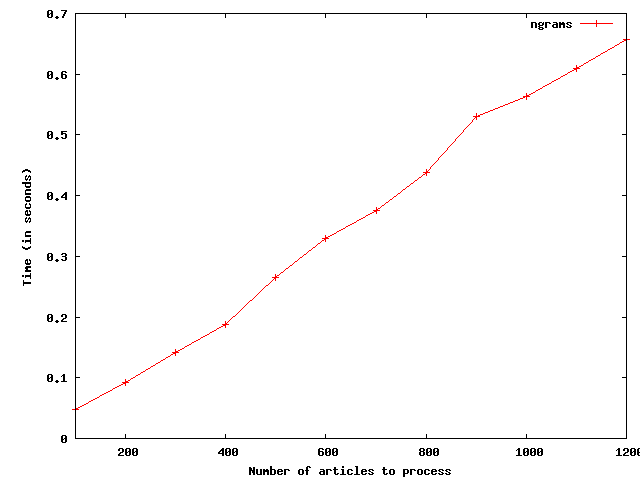
\includegraphics[width=\textwidth]{tabeller/ngram.png}\\
\caption{Time for n-gram creation\label{fig:ngram}}
\end{figure}

\subsubsection{Decide authors}

The horizontal values are the number of articles in the corpora, while the vertical values are the amount of articles that have to be attributed.\\
\begin{tabular}{|c|c|c|c|c|c|c|c|c|c|c|c|c|c|}
\hline 
 & 100 & 200 & 300 & 400 & 500 & 600 & 700 & 800 & 900 & 1000 & 1100 & 1200\\ 
\hline 
100 & 55.20 & 79.24 & 100.7 & 113.7 & 127.7 & 138.9 & 152.2 & 160.5 & 170.3 & 184.5 & 193.5 & 203.4\\ 
\hline 
200 & 104.5 & 150.7 & 192.0 & 217.7 & 244.2 & 265.5 & 290.4 & 305.9 & 324.3 & 351.5 & 368.8 & 387.6\\ 
\hline 
300 & 158.7 & 229.2 & 292.7 & 330.7 & 371.3 & 403.5 & 440.8 & 464.3 & 491.9 & 533.0 & 559.0 & 587.3\\ 
\hline 
400 & 212.1 & 306.8 & 391.2 & 442.1 & 496.4 & 539.2 & 588.6 & 619.7 & 656.1 & 710.5 & 745.1 & 782.6\\ 
\hline 
500 & 279.5 & 403.9 & 514.4 & 581.0 & 652.2 & 708.1 & 772.3 & 812.6 & 860.2 & 933.9 & 981.1 & 1032\\ 
\hline 
600 & 344.3 & 497.8 & 634.8 & 717.2 & 805.7 & 874.8 & 954.2 & 1004 & 1062 & 1150 & 1206 & 1267\\ 
\hline 
700 & 385.2 & 559.0 & 713.5 & 806.1 & 905.5 & 983.0 & 1072 & 1128 & 1193 & 1292 & 1355 & 1423\\ 
\hline 
800 & 449.3 & 650.7 & 830.8 & 939.5 & 1056 & 1148 & 1253 & 1318 & 1394 & 1510 & 1583 & 1663\\ 
\hline 
900 & 521.9 & 755.8 & 965.6 & 1092 & 1228 & 1333 & 1454 & 1529 & 1618 & 1751 & 1837 & 1930\\ 
\hline 
1000 & 576.8 & 836.1 & 1068 & 1208 & 1359 & 1475 & 1619 & 1705 & 1807 & 1966 & 2069 & 2175\\ 
\hline 
1100 & 615.9 & 891.6 & 1136 & 1285 & 1541 & 1664 & 1808 & 1898 & 2004 & 2164 & 2263 & 2374\\ 
\hline 
1200 & 663.2 & 961.7 & 1227 & 1387 & 1559 & 1694 & 1848 & 1947 & 2060 & 2231 & 2340 & 2457\\ 
\hline 
\end{tabular}

Figur \ref{fig:work}, which is based on the 12 horizontal line, clearly showes that the time required to attribute 1200 authors\footnote{I have choosen this particular line, since it is the final line, and given there should be any non-linear time increase from corpora size to corpora size, then this should be the line that showed it best} grows lineary witht the amount of posts in the corpora. 

\begin{figure}[!hbp]
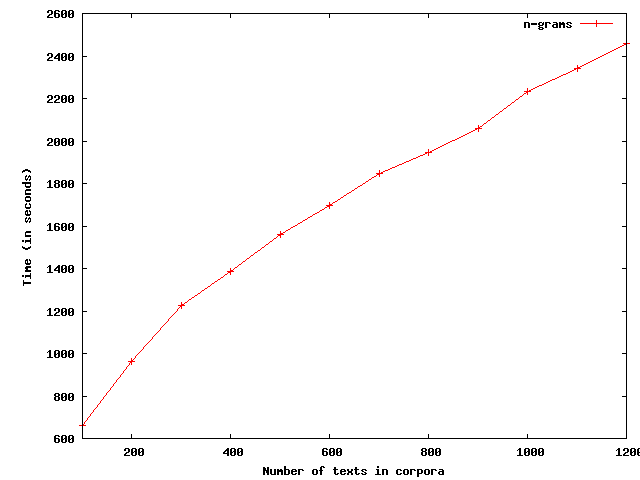
\includegraphics[width=\textwidth]{tabeller/work.png}
\caption{Time for article attribution with 1200 articles \label{fig:work}}
\end{figure}
